\section{Framework}

Describe comms framework, plugin framework, and software
development practices.

\subsection{Communications Framework}\label{SecComms}

The \ngrm\ architecture is hierarchical and recursive
(\ref{ReqsHiLevFun}, req. 4.1).
A root instance of \ngrm\ contains all the
idle resources.  A job spawned by the root instance contains
its own \ngrm\ instance, which may in turn spawn jobs, ad infinitum.
When a job terminates, the job's instance terminates and resources
return to the parent instance.

The communications framework supports this architecture by
establishing a {\em comms session} to contain each \ngrm\ instance.
The framework enables secure, scalable communication
within a comms session, limits communication between sessions,
and allows new comms sessions to be created, resized, destroyed,
and monitored by existing ones in a parent-child relationship.

A comms session is only ``aware'' of its parent and offspring.
Any communication between siblings would have to be orchestrated by
the parent.  This abstraction should encourage higher level software
to be built that can operate at any level of recursion, thus improving
testability and facilitating research.

The communications framework consists of three main layers:
the IP transport, comms toolkit, and comms message broker, shown
in Figure~\ref{FigCommsLayers}.  Layering is not rigid;
that is, higher level \ngrm\ components can use any of the
layers directly as appropriate.

\begin{figure}
\begin{minipage}[b]{0.45\linewidth}
\centering
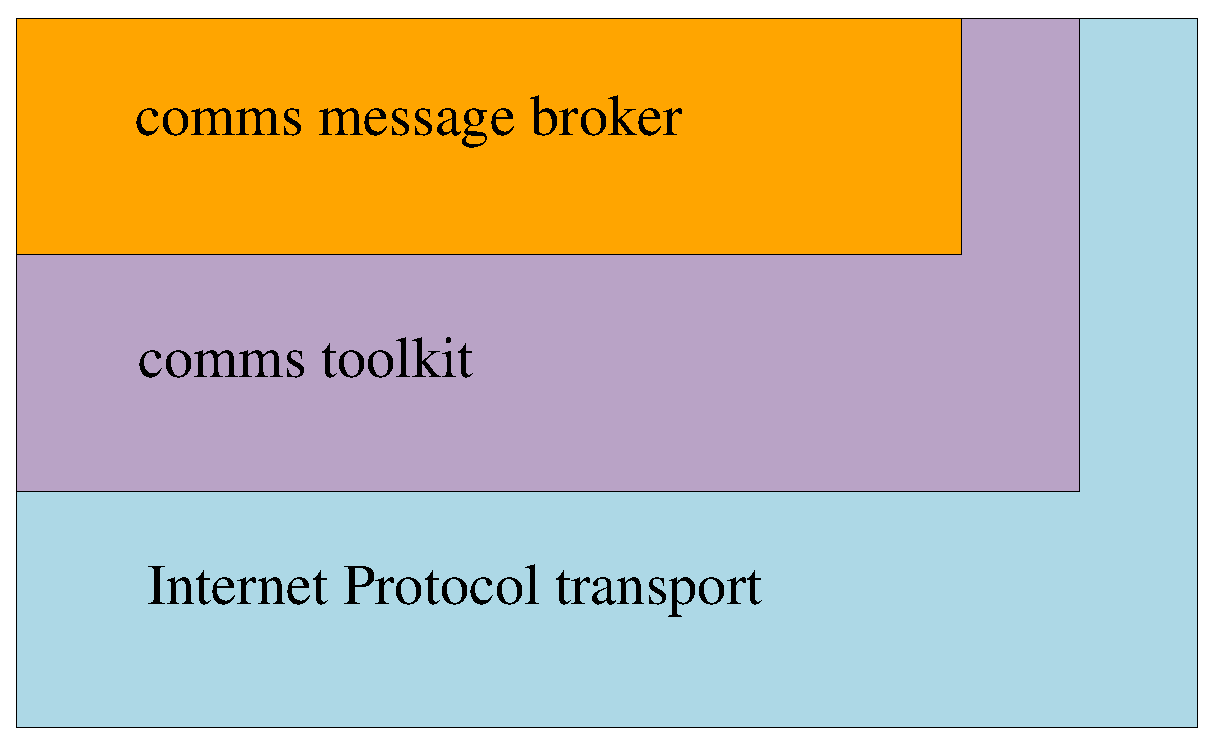
\includegraphics[scale=0.30]{../fig/comms.eps}
\caption{Comms Framework Layers}
\label{FigCommsLayers}
\end{minipage}
\hspace{0.5cm}
\begin{minipage}[b]{0.45\linewidth}
\centering
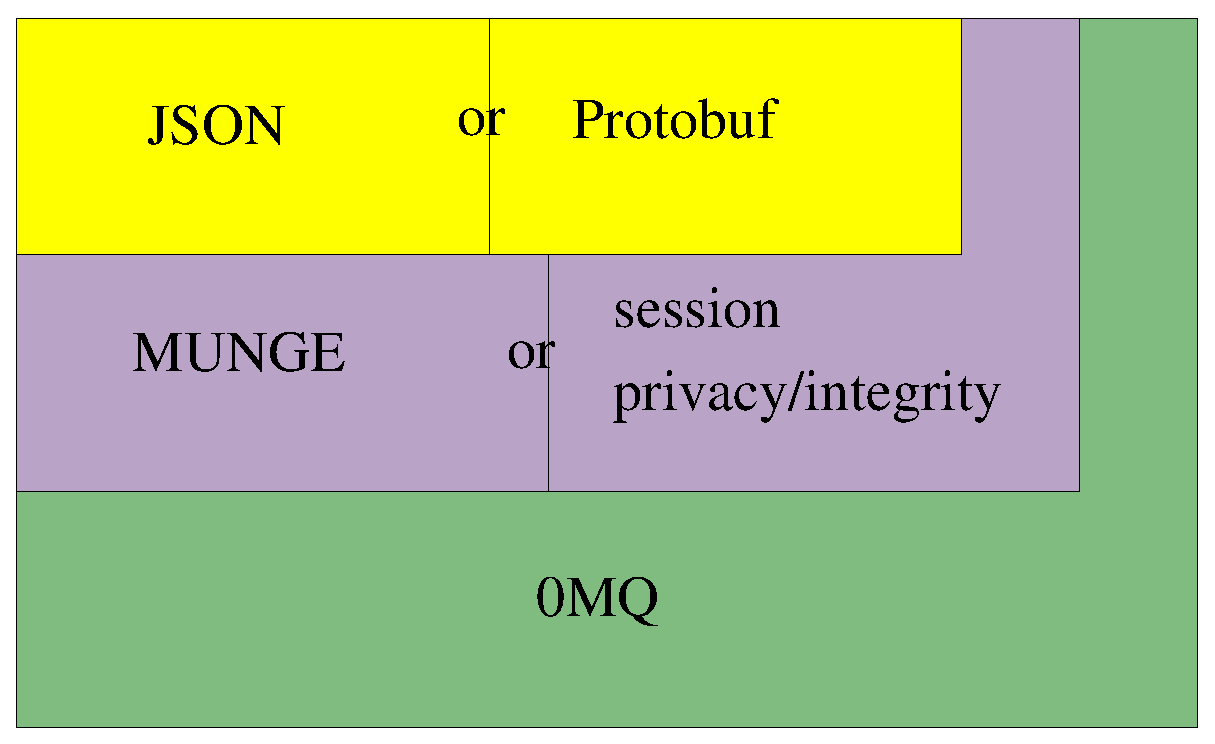
\includegraphics[scale=0.30]{../fig/commstk.eps}
\caption{Comms Toolkit Layers}
\label{FigCommsTK}
\end{minipage}
\end{figure}

\subsubsection{Internet Protocol Transport}

The \ngrm\ comms framework is layered upon IP, and presumes
complete IP level unicast and multicast connectivity, so that any
collection of nodes can be wired up in a comms session without
the need to re-implement the equivalent of IP routing within
the framework.\footnote{Building a reliable 100K node IP internetwork
is a solved problem.} 
The addressing, routing, and subnetting of this IP network is beyond of
scope of \ngrm, except that its design should introduce no single
points of failure (\ref{ReqsHiLevFun}, req. 1.2), should be protected
from external intrusion, and should avoid performance bottlenecks which
would unnecessarily constrain the resource manager's node selection options.

The comms framework should support communication over multiple
(fully-routed) network planes, for example using either a management
ethernet or IP-over-IB or both according to the performance/reliability
requirements of the particular application.

Dynamic unicast IP address allocation must be available to support
dynamically created virtual nodes (Linux containers launched with
virtual network interfaces).  Similarly,
dynamic multicast address allocation must be available to support
private multicast groups within dynamically created comms sessions.
These requirements can be addressed by existing technology such as
DHCP\cite{rfc2131} and MADCAP\cite{rfc2730}.

A private DNS\cite{rfc1034} is used by the comms framework to
map a hierarchical namespace to the comms session hierarchy.
The root comms session has the root domain name, e.g. ``{\tt \ngrm.}'',
and the root server contains address records for all hosts in the domain, e.g.
``{\tt n1.\ngrm}'', ``{\tt n2.\ngrm}'',..., ``{\tt n99999.\ngrm}''.
Comms sessions spawned by the root session get their own sub-domain, e.g.
``{\tt s1.\ngrm}'', ``{\tt s2.\ngrm}'', ``{\tt s3.\ngrm}'',
and contain address records for the nodes assigned to them, e.g.
``{\tt n1.s1.\ngrm}'', ``{\tt n2.s1.\ngrm}'', ``{\tt n3.s1.\ngrm}''.
Sub-domains are created for each level of comms session recursion.
Each session runs a set of DNS servers for its domain.
When a node joins a new session, its DNS resolver is reconfigured to use
the session DNS servers and to search the session's DNS domain first,
thus each level of session overlays a new set of names over
the root session's that provides job-centric naming uniformity.
DNS SRV records\cite{rfc2782} provide a rudimentary service location
brokerage within the session.
Well understood techniques for DNS fault tolerance,
caching, and dynamic reconfiguration are leveraged to scale performance
in large sessions such as the root session.

A comms session could optionally be spawned inside a virtual private
network (\ref{ReqsUseCases}, UC21) such that IP communication
is limited to within the comms session.  IPsec\cite{rfc2401} with
a pre-shared session key could be used to provide session integrity and
privacy at the IP layer if desired.

\subsubsection{Comms Toolkit}

The framework provides a toolkit for sending and receiving
protocol messages privately and securely within a session,
with the goals of providing a robust foundation for \ngrm\ components
and promoting rapid development, code reuse, and interoperability.
The toolkit includes messaging libraries,
protocol encoding/decoding libraries, and security options.
Toolkit pieces can be mixed and matched according to application
requirements.  We may cull the comms toolkit as we learn more
about the pieces while prototyping other \ngrm\ comopnents.

Two messaging approaches of interest are 0MQ\cite{ZMQGuide} and
SCTP\cite{SCTP}.
0MQ provides the ability to manipulate opaque, multipart messages,
and carry them across various transports, including TCP and
PGM\cite{rfc3208} (reliable multicast), using a socket-like API.
0MQ sockets can exchange messages using patterns including
REQ-REP (RPC), PUB-SUB, and PUSH-PULL (message stream).
0MQ can be used to build applications or custom message brokers.
Complex message routing topologies such as tree-based overlay networks
(Figure~\ref{FigZmqTBON}) can be built from simple components.
0MQ has a large number of language bindings.

SCTP is an IETF-standardized, message-oriented transport developed
in the telephony world with an implementation in the Linux kernel.
It offers multi-streaming, the bundling of {\em streams} in one
{\em association} (connection).  Individual streams can be configured for
different ordering and reliability semantics.  SCTP supports
multi-homing for reliability and congestion avoidance, and
can transparently generate and check an HMAC for messages using a
pre-shared key to implement message integrity.  Unlike 0MQ, SCTP is
connection-based and does not implement a standardized reliable multicast
mode.

\begin{figure}
\centering
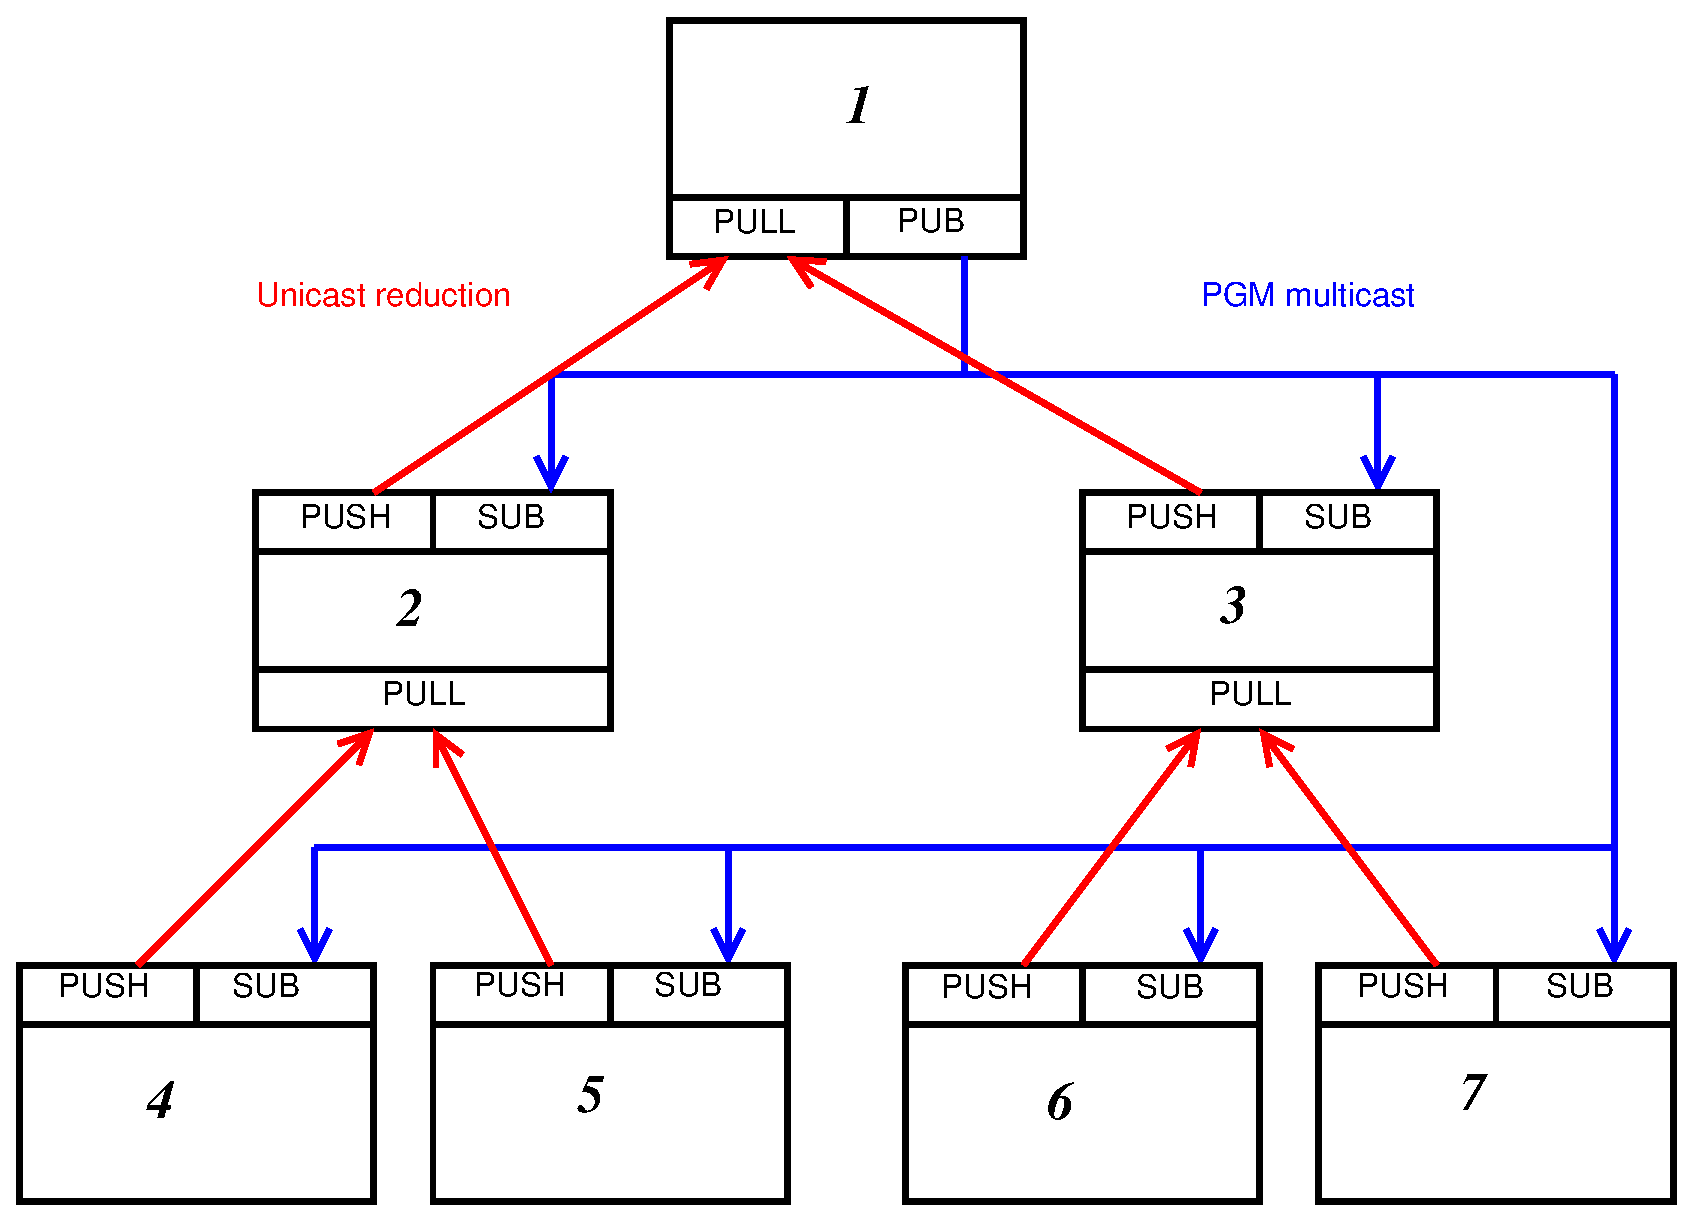
\includegraphics[scale=0.35]{../fig/zmqtbon.eps}
\caption{Tree Based Overlay Network Over 0MQ}
\label{FigZmqTBON}
\end{figure}

Two widely used methods of encoding data in messages are
JSON\cite{rfc4627} 
and Protocol Buffers\cite{Protobuf}.
JSON is a self-describing format
that supports protocol evolution without recompiling endpoints.  It has
many language bindings but it is also space-inefficient and slow.
Protocol Buffers is a compiled format that supports
only limited protocol evolution without recompilation.  It has relatively
fewer language bindings than JSON but is space-efficient and fast.
Depending on the application either may be appropriate.

Messages can be secured with a session-wide security context.
Each comms session is allocated a {\em session key} by its parent\footnote{
The root comms session obtains its session key out of band.}
which is used for establishing a shared security context
for messages exchanged within the comms session.
The shared security context allows communicating entities to have integrity
and privacy (from children, siblings, and their children)
without the overhead
of a key exchange for each pair of communicating endpoints.
This is especially useful for non point-to-point comms patterns such as PUB-SUB.
The parent retains state about its offspring including their session keys.
Children forget their parent's key;  thus as comms sessions recurse,
parents get privacy from children but not the reverse.
An application acting as a gateway between parent and child would use
the child's session key as it is known by both parent and child.

Alternatively, messages can be enclosed as payload in a MUNGE\cite{MUNGE}
credential when authentication of the sending user is required.
This also provides intergrity and privacy for the message that
is robust to threats from within the comms session.
In order for this to work, \ngrm's comms framework must operate within a
single MUNGE security realm,\footnote{MUNGE must acquire the ability
to update its shared secret without introducing downtime. FIXME: ref bug\#}
which implies a single single administrative domain with consistent
user and group identities.

\subsubsection{Comms Message Broker}\label{SecCommsCMB}

Within a comms session, a distributed comms message broker (CMB)
is established to provide basic session services.
The CMB is responsible for launching new sessions,
managing session membership,
detecting and adapting to session node failures,
providing a basic event messaging system,
and starting other \ngrm\ components.

\paragraph{Architecture}
The CMB is a distributed service with nodes interconnected in a topology
that is to be determined.
A distinguished {\em control node} serves as the heart of the CMB.
The control node is distinguished because it alone communicates with
the parent session, and it holds the master copy of the session state.
For fault tolerance, there is a primary and backup control node for each
each session, with the parent CMB initiating any takeover.
Interfaces exposed by the control node to the parent are always passive;
that is, the parent initiates connections and makes requests or subscribes
to events, and the child control node responds or publishes events.

\paragraph{Session State}
The CMB implements a simple key-value store to manage the
internal state enumerated in Table~\ref{TabCMBState}.
The session state for the largest session is small enough to easily
fit in memory.
The master state lives on the control node.
Slave caches on other nodes are loosely consistent with the master copy:
reads may utilize a local or peer cache;
writes are through to the control node.
Each write on the control node updates the key's generation number,
its value, and triggers a state update event which
can be used to update caches and synchronize other software using the
state.

\begin{table}
  \centering
  \begin{tabular}{| l | p{0.6\textwidth} |}\hline
  \textbf{Name} & \textbf{Description} \\
  \hline
  cmb.cred = $key$ &
        My session key.\\
  cmb.fqdn = $name$ &
        Fully qualified domain name for the session.\\
  cmb.nodeset = $nodelist$ &
        List of my nodes.\\
  cmb.addrs.$node$ = $addrs$ &
        List of addresses for $node$, for forming DNS address records.\\
  cmb.topology.up.$node$ = $nodelist$ & 
        Upward peers for $node$ in CMB topology.\\
  cmb.topology.dn.$node$ = $nodelist$ &
        Downward peers for $node$ in CMB topology.\\
  cmb.alive.$node$ = $yes|no$ &
        Liveness for $node$.\\
  cmb.alloc.$node$ = $yes|no$ &
        Allocation status for $node$.\\
  cmb.attrs.$node$ = $attrlist$ &
	Role attributes assigned to $node$, e.g. ``dns'' and ``control''.\\
  cmb.subscribe.$key$ = $nodelist$ &
        List of nodes subscribed to $key$.\\
  cmb.exec = $cmdline$ &
        Executable to bootstrap on each node.\\
  \hline
  cmb.child.sessions = $sessions$ &
        List of active child sessions.\\
  cmb.child.$session$.cred = $key$ &
        Child sesion key.\\
  cmb.child.$session$.control = $nodelist$ &
        Control node(s) for $session$.\\
  cmb.child.$session$.dns = $nodelist$ &
        DNS server nodes for $session$, for forming DNS NS records.\\
  \hline
  \end{tabular}
  \caption{Comms Message Broker State}
  \label{TabCMBState}
\end{table}

\paragraph{Event Messaging}
The CMB implements a session-wide event messaging service.
Clients of the CMB on any node can publish a $(key, message)$ event tuple.
Other clients can subscribe to events by key.  The CMB ensures that
event messages are routed internally from publishers to subscribers.
The event service is reliable, and for events originating on the same node,
sequenced for in-order delivery.
Events are not queued for late subscribers.
There is a special {\tt event.sched.trigger} event sent out periodically
to synchronize the CMB's internal functions (and those of any other
subscribers to the event) across the session with the goal of minimizing
disruption to bulk-synchronous workloads running within the session.

\paragraph{Session Membership}
The CMB maintains the current {\em nodeset} as part of the session state.
The CMB arranges for the nodeset to be mirrored in private DNS servers
serving up the session's subdomain.
The nodeset may grow or shrink in response to higher level software
allocating/freeing nodes from the parent, or creating/destroying 
virtual nodes within the session.
Nodeset updates will be accompanied by internal topology updates, provided by
the software making the nodeset change or by the CMB itself depending
on the situation.
State update events will be published for the nodeset and topology changes.
While nodes are allocated to a session, they remain in the parent nodeset,
tagged as {\em allocated}.  They forget the parent's session state and key.
When nodes are freed back to the parent, the parent CMB, having subscribed
to the child's nodeset update events, contacts the freed node (using the
child session key) and brings it back online in the parent sesssion.  

\paragraph{Liveness Monitoring}
The CMB maintains the {\em liveness} of its nodes as part
of the session state.
Liveness is assessed by forcing member nodes to communicate with the CMB
at minimum intervals, synchronized by the aforementioned trigger event.
If the CMB has not heard from a node for some number
of trigger periods, it is marked down.
If it finally is heard from, it is marked {\em up}.
In some cases the CMB control node may adjust its internal topology
to account for such changes.
As described above, session state changes trigger state change events.
Higher level software wishing to react to node liveness changes can
subscribe to state change events.
The parent continues to track liveness of nodes allocated to a child by
subscribing to liveness updates via the child's control node.  A trivial
utility that asks the CMB for a list of down nodes in the current session
can be written that works equally well at any level of recursion,
even at the level of the root session.

\paragraph{Node Bootstrap}
A cold started node (or restarted CMB daemon) joins the root session,
obtaining the root session key and the identity of a peer to copy the
session state from out of band in a secure manner.
If the CMB is cold starting after crashing while assigned to
a session other than the root, the CMB of the root and subsequent owning
sessions re-add the node from child to child until there are no children
left or it is evicted according to the policy of an owning session.

\paragraph{Executable Bootstrap}
In order to bootstrap other \ngrm\ components, the CMB daemon, upon
joining a new session, launches a single process on each node,
determined by the {\tt cmb.exec} state variable.
This process is terminated when the node alters its session membership
to join a child session or return to a parent session.
If the process terminates early, an event is generated.

%\begin{figure}
%\centering
%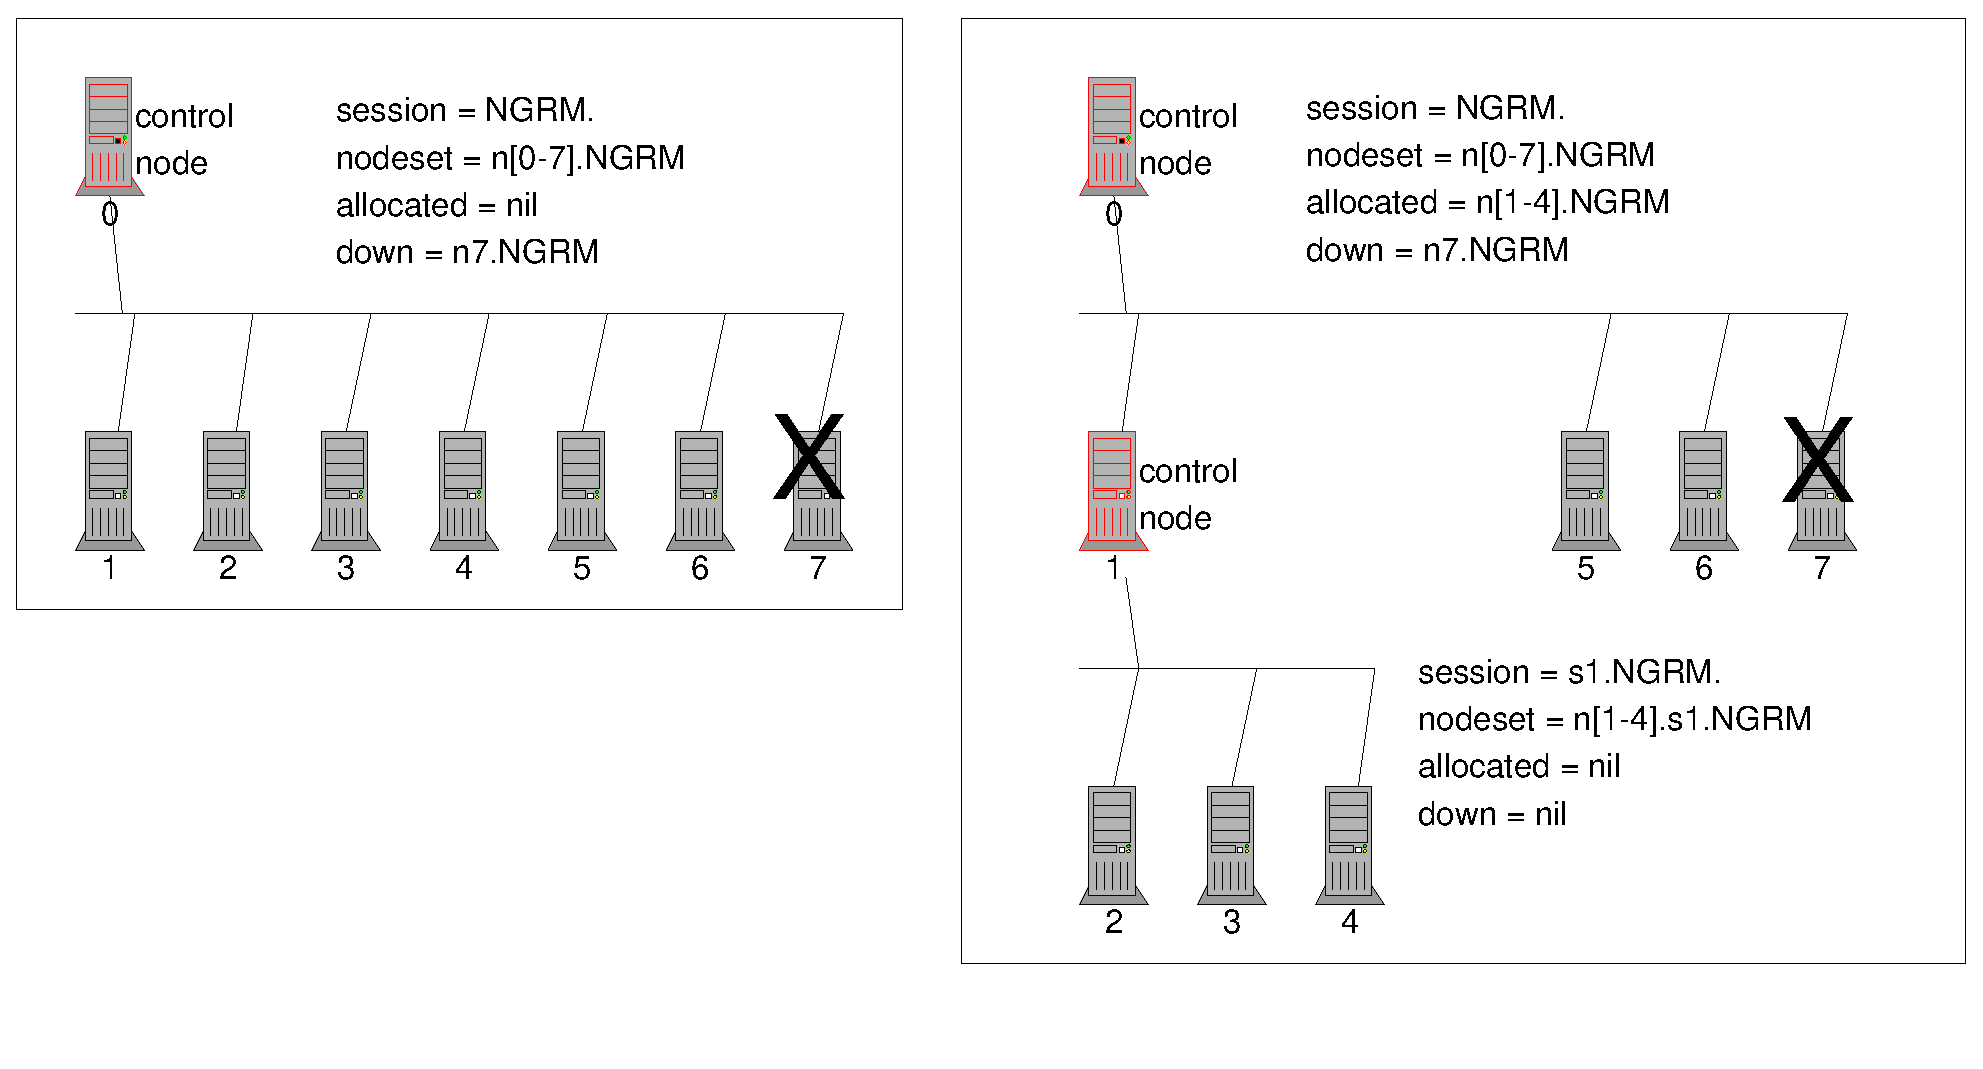
\includegraphics[scale=0.50]{../fig/cmb.eps}
%\caption{Comms Message Broker Spawning a New Comms Session}
%\label{FigCMBSpawn}
%\end{figure}

\paragraph{Session Creation}
The CMB is responsible for the creation of
child comms sessions.
%as shown in Figure~\ref{FigCMBSpawn}.
A child session is created by building the child session state,
updating the current (parent) session state, then sending the
child control node(s) the full session state, and the rest of the nodes
just the new session key and sufficient information to wire up to their
peers in the internal toplogy.
The DNS is updated in the parent to delegate authority
for the new subdomain to the child's DNS servers.
DNS servers are bootstrapped in the child, and the resolver is updated
on member nodes to reflect the new session.

\paragraph{Session Destruction}
The CMB destroys a child comms session by sending a message to the child's
control node requesting that a shutdown event be sent out session wide.
As nodes leave the child nodeset, the parent reclaims them as described 
above in the Session Membership paragraph.
If something goes wrong, the parent can short-circuit the ``clean shutdown''
and actively reclaim nodes as above, as though they had already left the
child nodeset.
The DNS is updated in the parent to remove references to the session's
subdomain.
